% !TEX TS-program = pdflatex
% !TEX encoding = UTF-8 Unicode
% !BIB TS-program = biber
% !BIB program = biber

\documentclass[12pt]{article}

%%% PAGE DIMENSIONS
\usepackage[margin=2.54cm]{geometry}
\geometry{a4paper} 
% \usepackage{caption}
% \usepackage{subcaption}
\usepackage{graphicx} % For better graphics
\usepackage{pdfpages} % To insert pdfs into the library
\usepackage{tikz}
\usepackage{wrapfig}
\usepackage{siunitx}

%%% PACKAGES
\usepackage{booktabs} % for much better looking tables
\usepackage{amsmath} % for better maths
\usepackage{paralist} % very flexible & customisable lists (eg. enumerate/itemize, etc.)
\usepackage{verbatim} % adds environment for commenting out blocks of text & for better verbatim
\usepackage{subfig} % make it possible to include more than one captioned figure/table in a single float
\usepackage[framed,numbered]{matlab-prettifier} % enable inserting matlab code.
\usepackage[parfill]{parskip}
%\addtolength{\jot}{1em}
\usepackage{amssymb}
\usepackage{cancel}
\usepackage{color}
\usepackage{listings}
% Create Listing Colours
\usepackage{xcolor}

% \definecolor{codegreen}{RGB}{0,255,0}
% \definecolor{codegray}{RGB}{105,105,105}
% \definecolor{codepurple}{RGB}{138,43,226}
% \definecolor{backcolour}{RGB}{255,255,255}
\definecolor{codegreen}{rgb}{0,0.6,0}
\definecolor{codegray}{rgb}{0.5,0.5,0.5}
\definecolor{codepurple}{rgb}{0.58,0,0.82}
\definecolor{backcolour}{rgb}{0.95,0.95,0.92}

\lstdefinestyle{mystyle}{
    backgroundcolor=\color{backcolour},   
    commentstyle=\color{codegreen},
    keywordstyle=\color{magenta},
    numberstyle=\tiny\color{codegray},
    stringstyle=\color{codepurple},
    basicstyle=\ttfamily\footnotesize,
    breakatwhitespace=false,         
    breaklines=true,                 
    captionpos=b,                    
    keepspaces=true,                 
    numbers=left,                    
    numbersep=5pt,                  
    showspaces=false,                
    showstringspaces=false,
    showtabs=false,                  
    tabsize=2
}
\lstset{style=mystyle}

\usepackage{multicol}
\usepackage{float}

% References
\usepackage[backend=biber,style = numeric]{biblatex}
\bibliography{sources}

%%% HEADERS & FOOTERS
\usepackage{fancyhdr} % This should be set AFTER setting up the page geometry
\setlength{\headheight}{15pt}
\pagestyle{fancy} % options: empty , plain , fancy
\renewcommand{\headrulewidth}{0pt} % customise the layout...
\lhead{University of Auckland}\chead{GOCPI}\rhead{Connor McDowall}
\lfoot{}\cfoot{\thepage}\rfoot{}

%%% SECTION TITLE APPEARANCE
\usepackage{sectsty}

%%% ToC (table of contents) APPEARANCE
\usepackage[nottoc,notlof,notlot]{tocbibind} % Put the bibliography in the ToC
\usepackage[titles,subfigure]{tocloft} % Alter the style of the Table of Contents
\renewcommand{\cftsecfont}{\rmfamily\mdseries\upshape}
\renewcommand{\cftsecpagefont}{\rmfamily\mdseries\upshape} % No bold!

%%% Hyperlinking 
\usepackage{hyperref}
\begin{document}
\begin{titlepage}
	\newcommand{\HRule}{\rule{\linewidth}{0.5mm}} % Defines a new command for horizontal lines, change thickness here
	
	\center
	
	%------------------------------------------------
	%	Headings
	%------------------------------------------------
	
	\textsc{\LARGE }\\[1.5cm] % Main heading such as the name of your university/college
	
	\textsc{\Large ENGSCI 700A/B}\\[0.5cm] % Major heading such as course name
	
	%------------------------------------------------
	%	Title
	%------------------------------------------------
	
	\HRule\\[0.5cm]
	
	{\huge\bfseries Research Compendium}\\[0.4cm] % Title of your document
	
	\HRule\\[0.5cm]
	
	%------------------------------------------------
	%	Author(s)
	%------------------------------------------------
	
	{\large\textit{Connor McDowall \\cmcd398 \\530913386}}\\
	
	%------------------------------------------------
	%	Date
	%------------------------------------------------
	
	\vfill\vfill\vfill % Position the date 3/4 down the remaining page
	
	{\large\today} % Date, change the \today to a set date if you want to be precise
	 
	%----------------------------------------------------------------------------------------
	
	\vfill % Push the date up 1/4 of the remaining page
	
\end{titlepage}
\tableofcontents
\listoffigures
\listoftables
\newpage
\section{Website}
\subsection{Version Two}
The website was improved using Jekyll, Ruby and Markdown technologies.
\textbf{You can access the website \href{https://connormcdowall.com/gocpi.html}{here}}
The following screenshots show the necessary sections of the website.
\subsection{Version One}
This html script was adapted from an W3 schools template to include key information about the project.
\begin{figure}[h]
    \centering
	\includegraphics[width=\textwidth]{W1.png}
	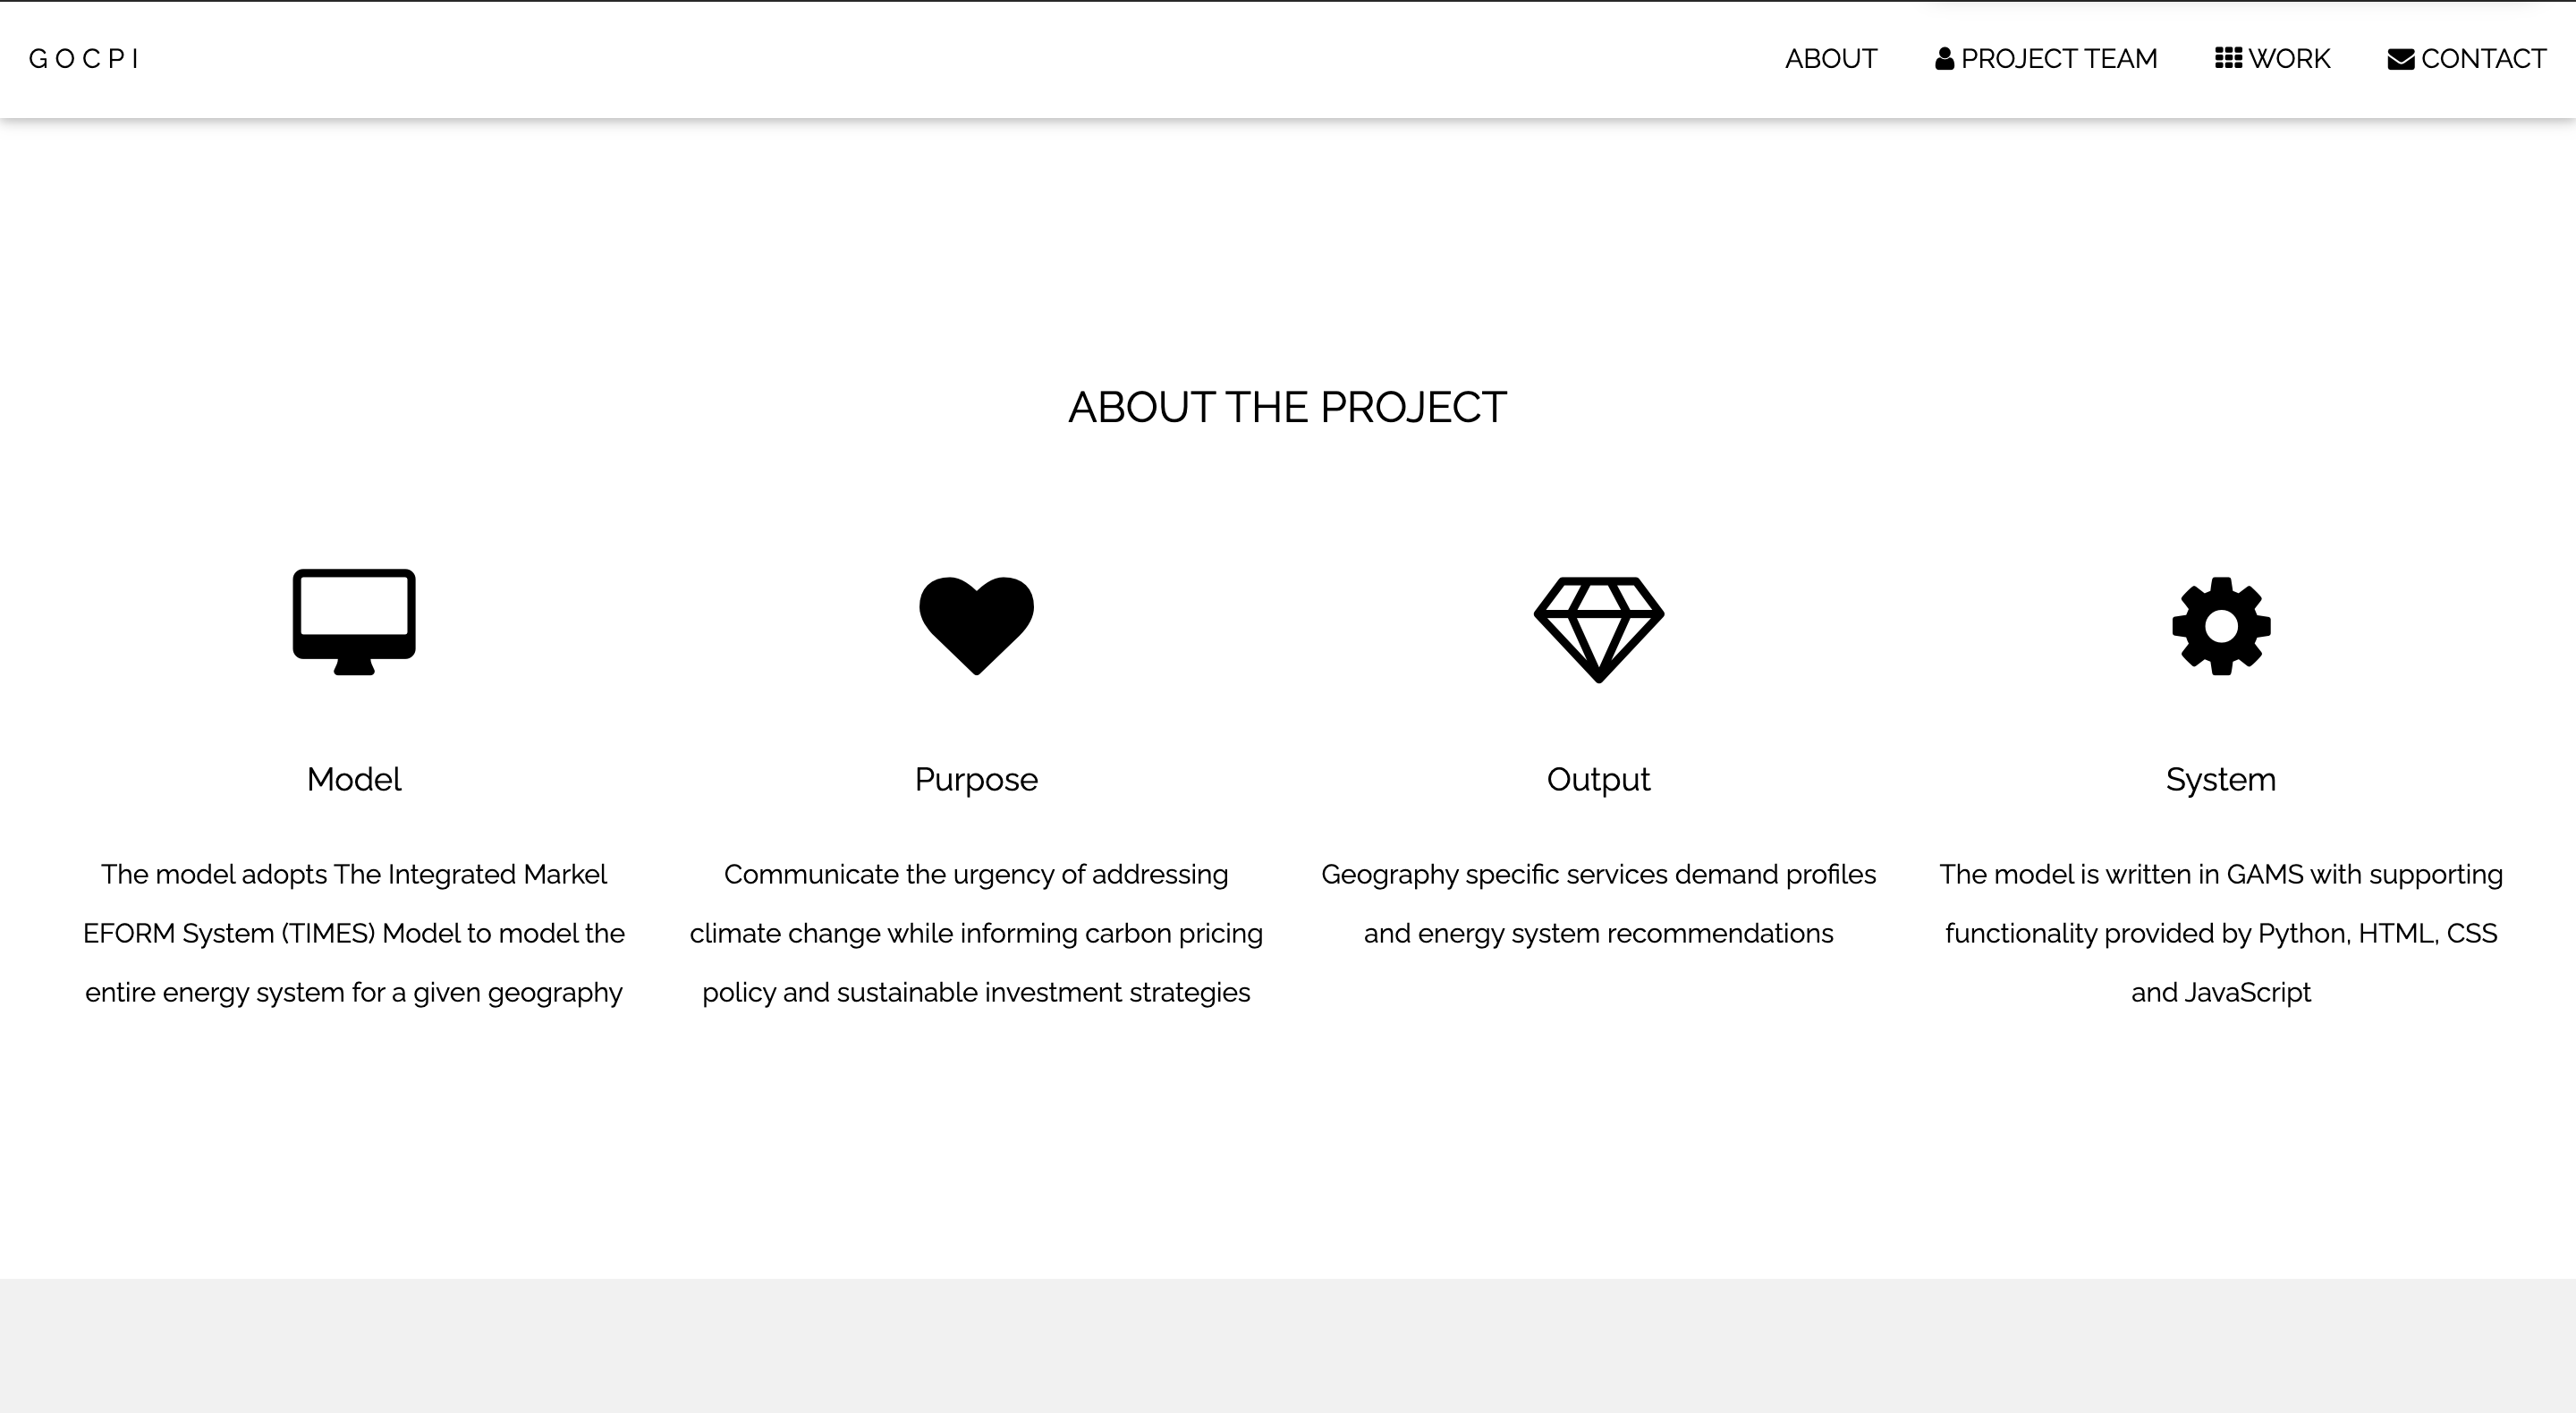
\includegraphics[width=\textwidth]{W2.png}
	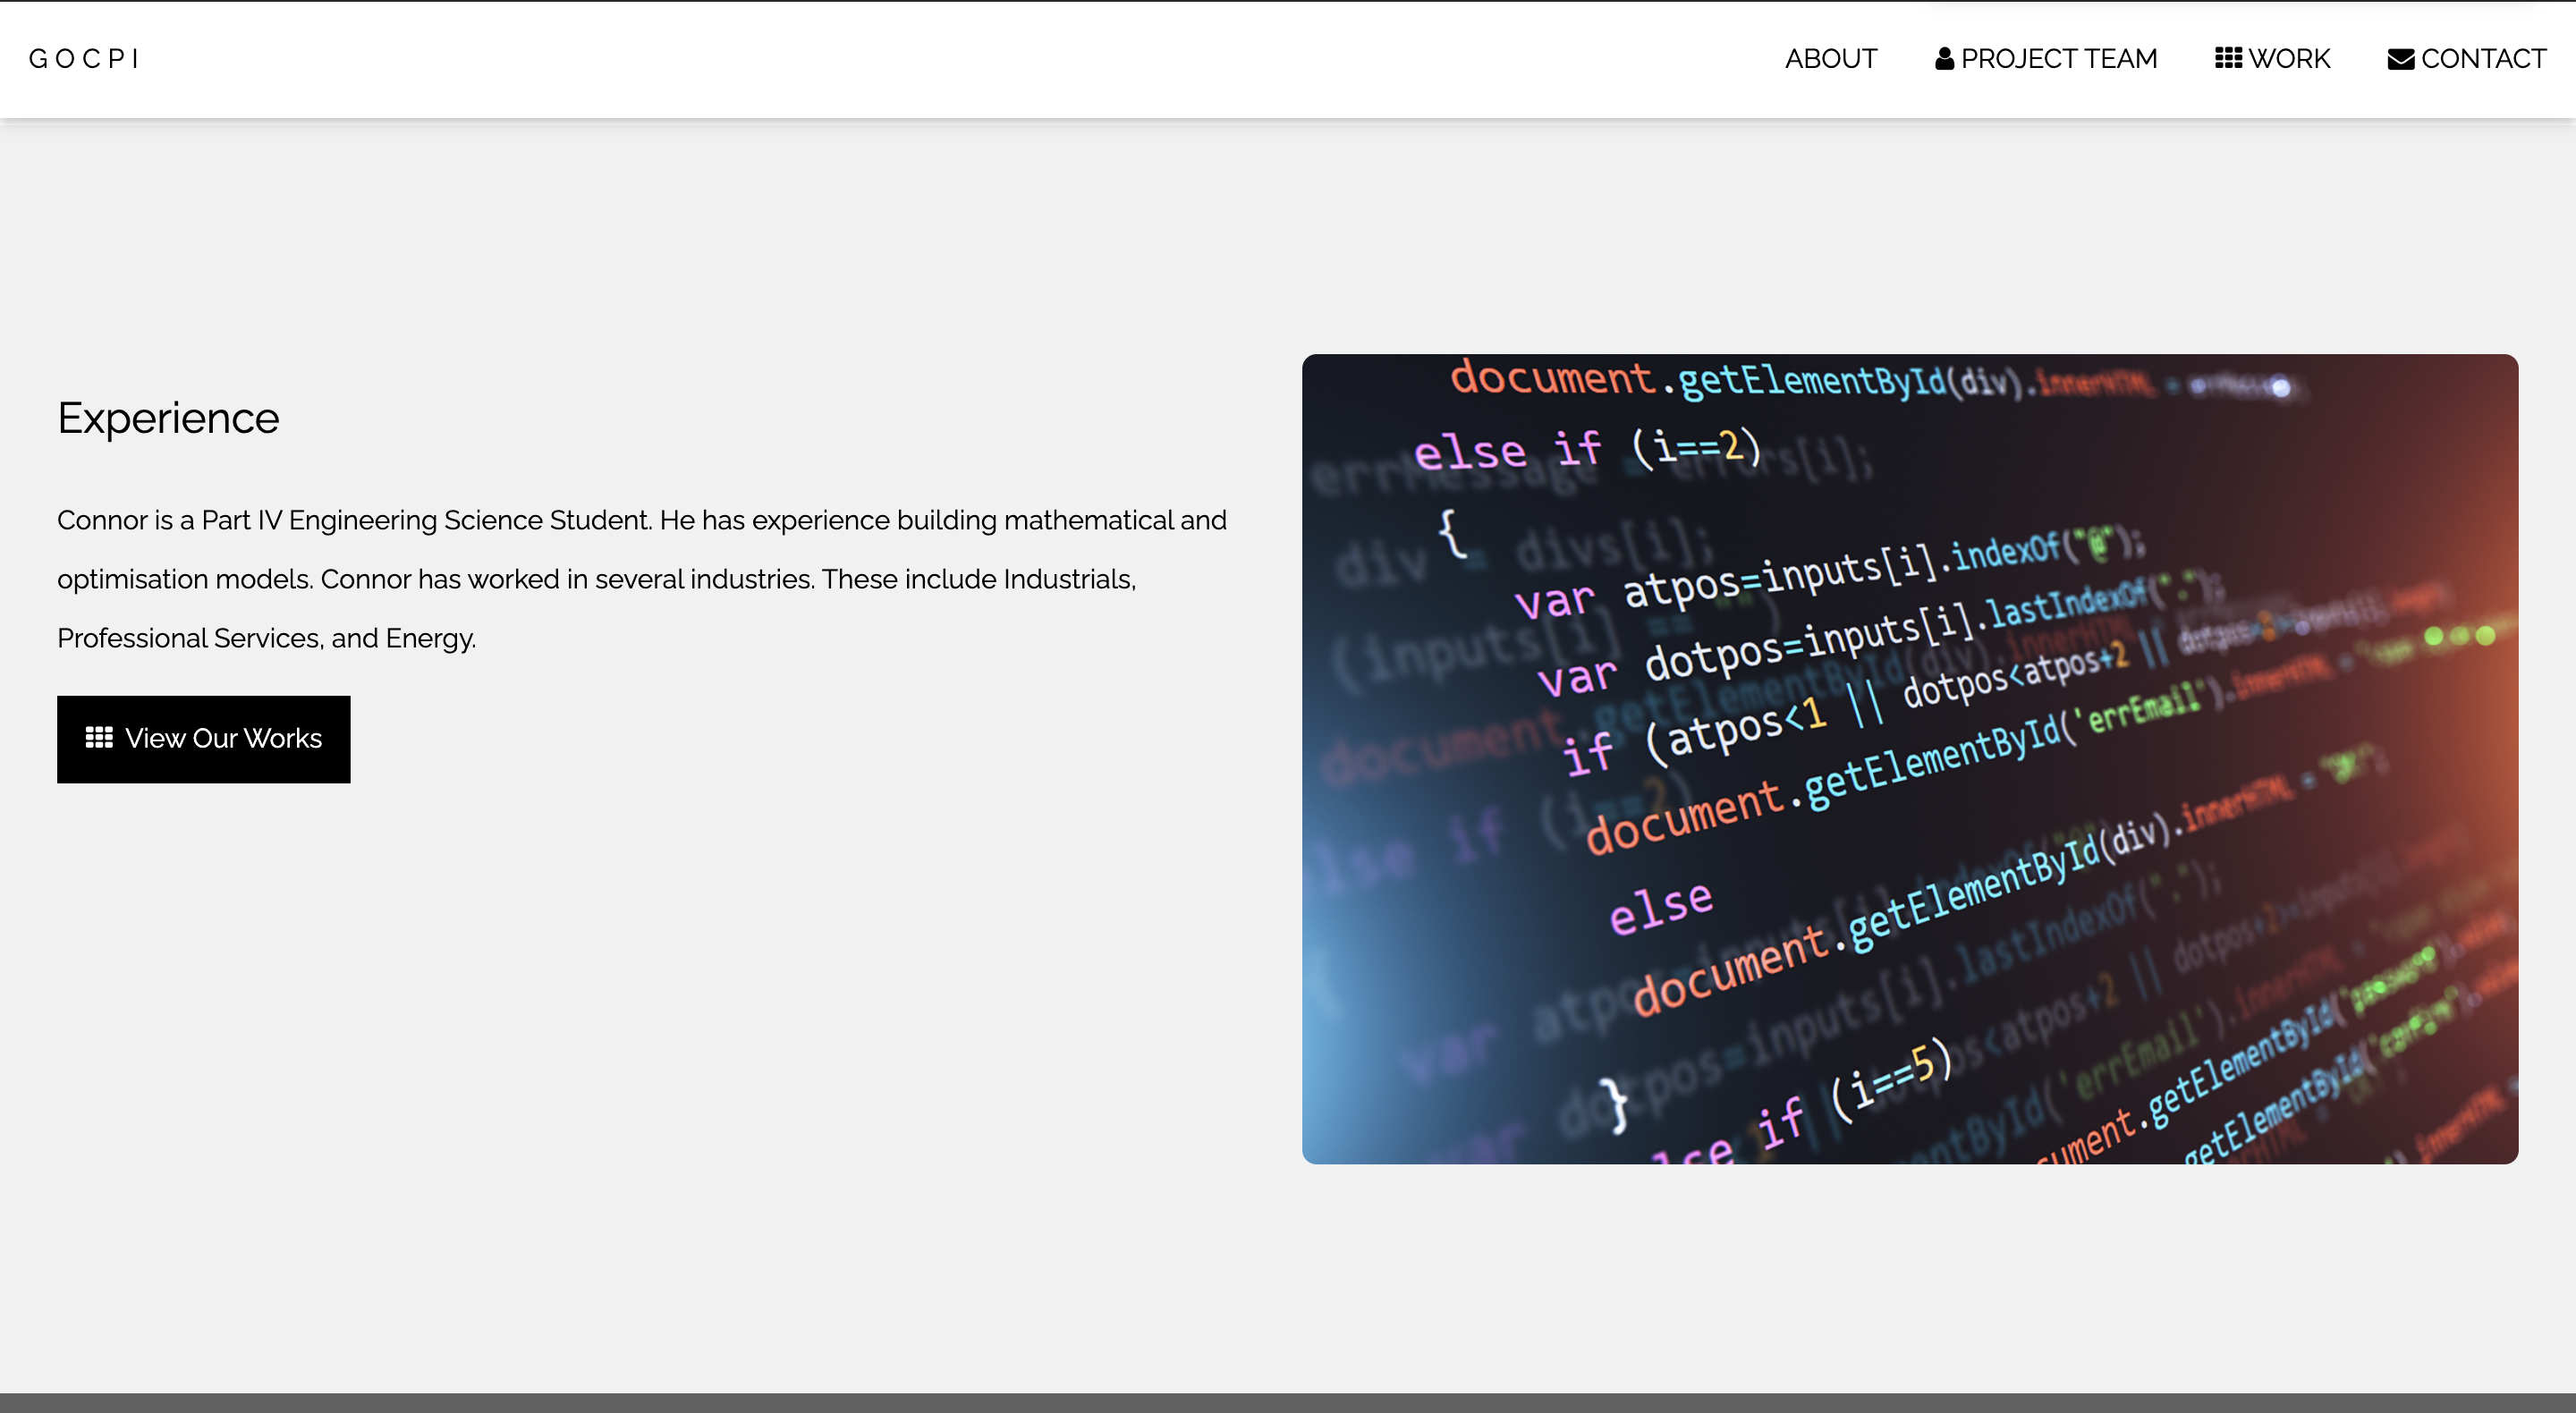
\includegraphics[width=\textwidth]{W3.png}
	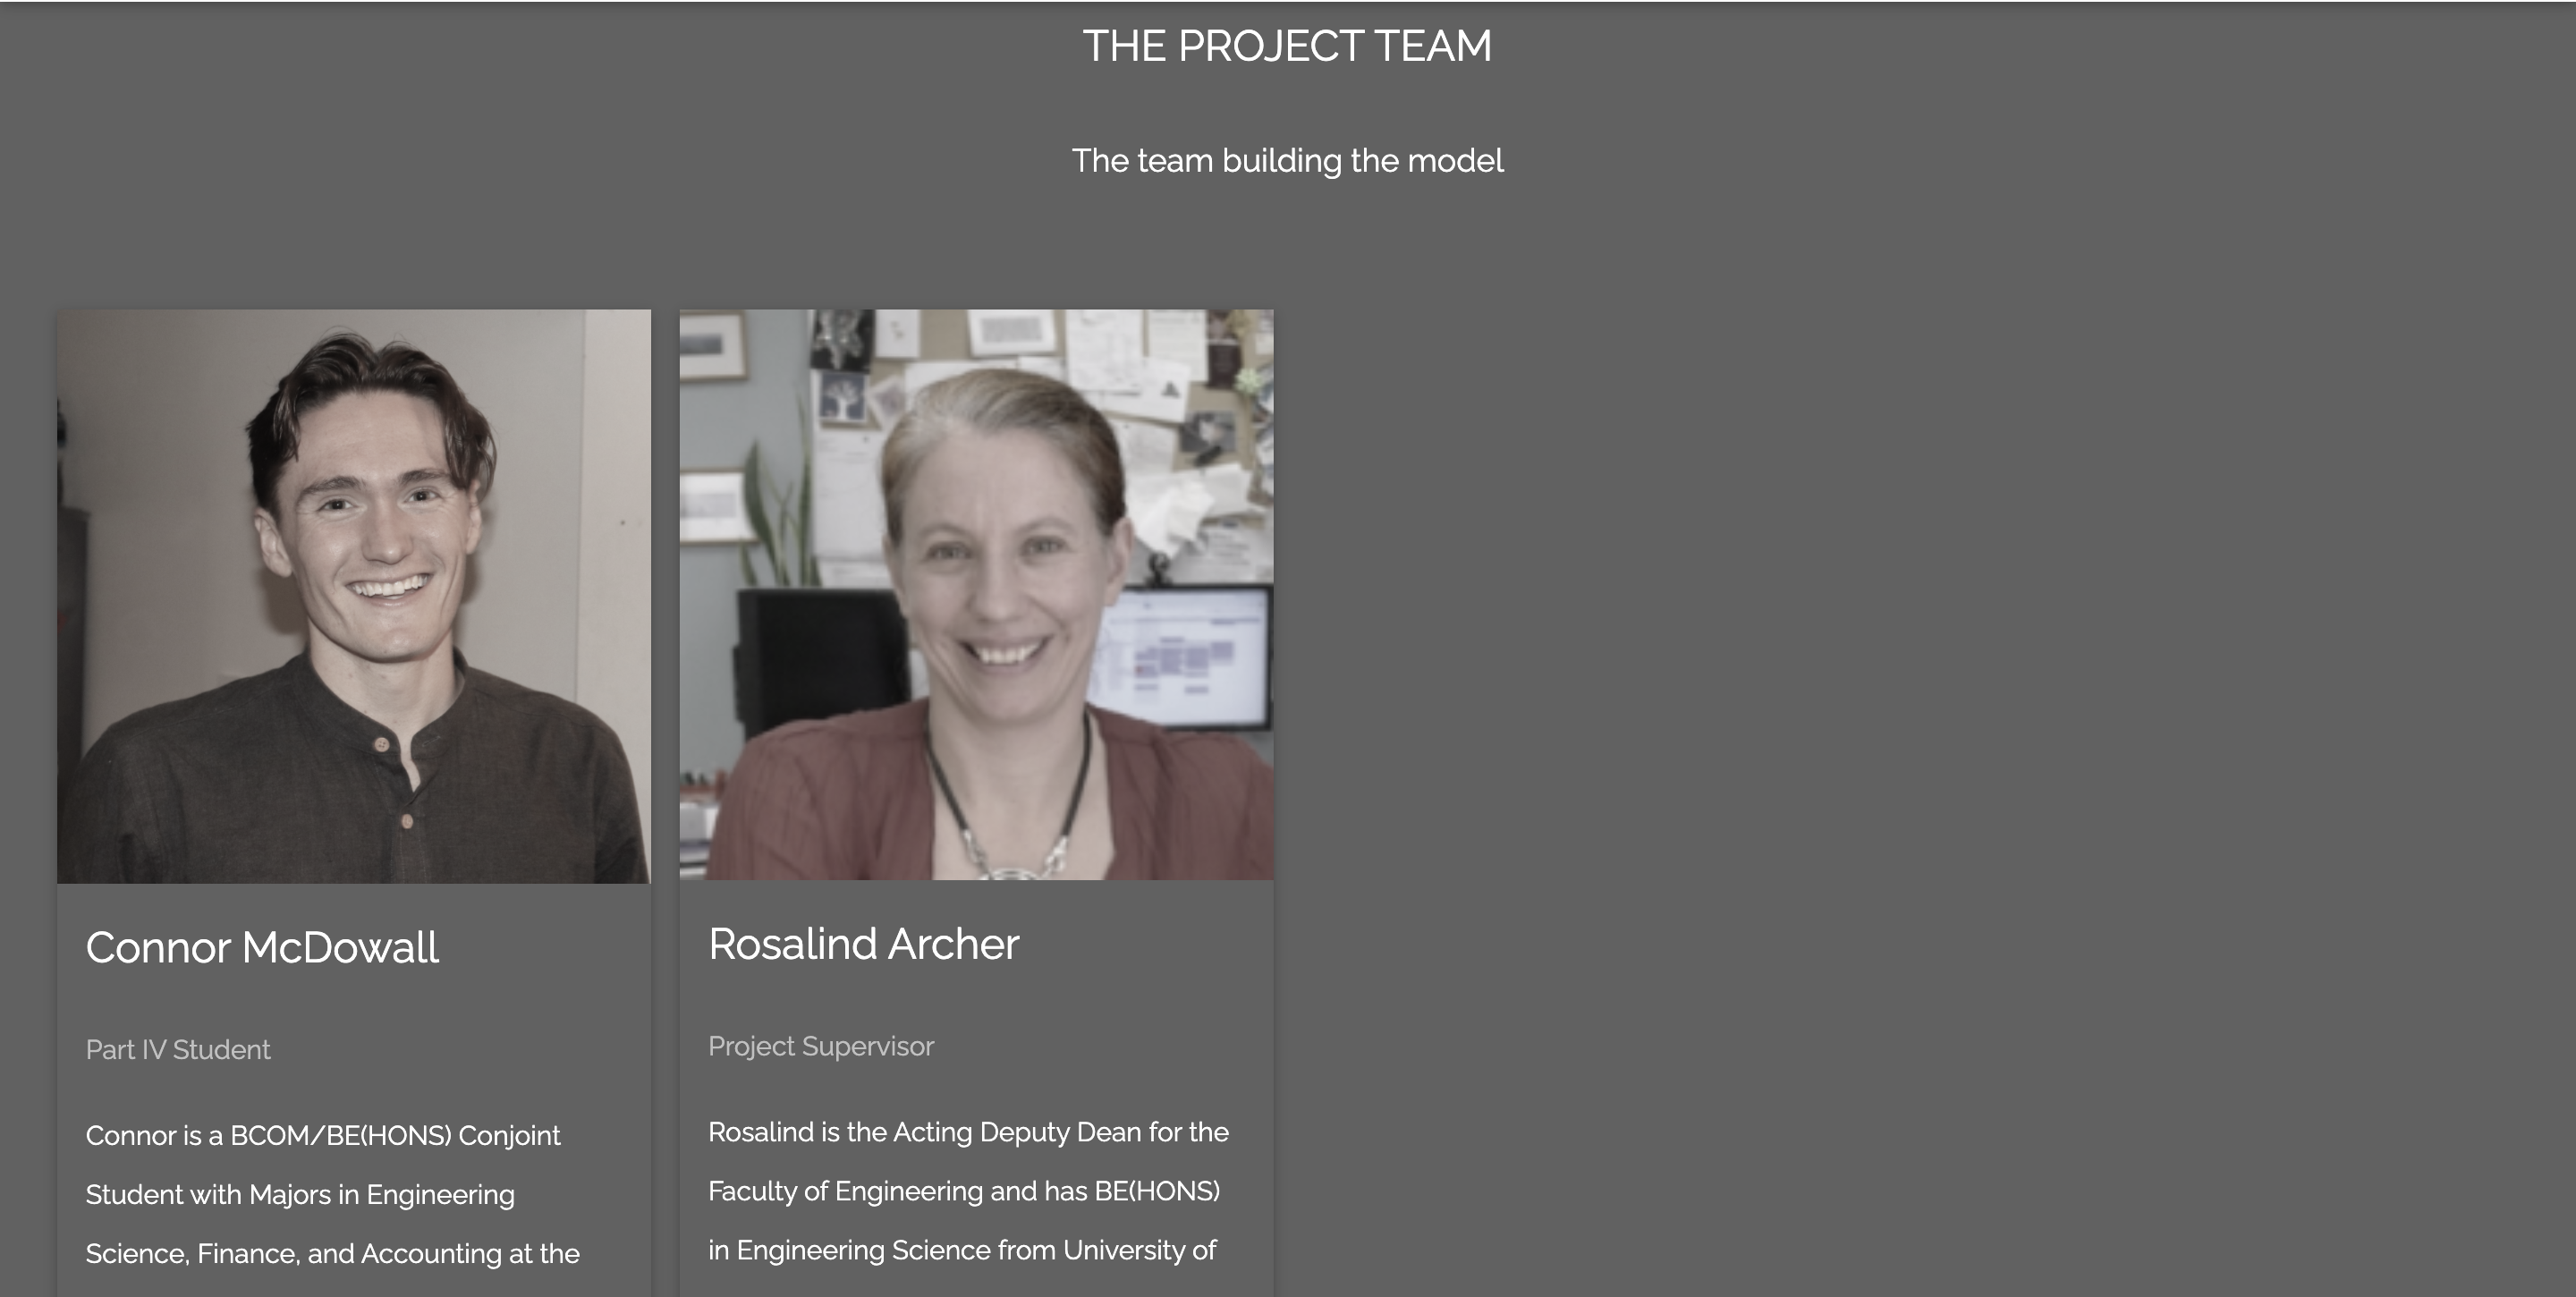
\includegraphics[width=\textwidth]{W4.png}
	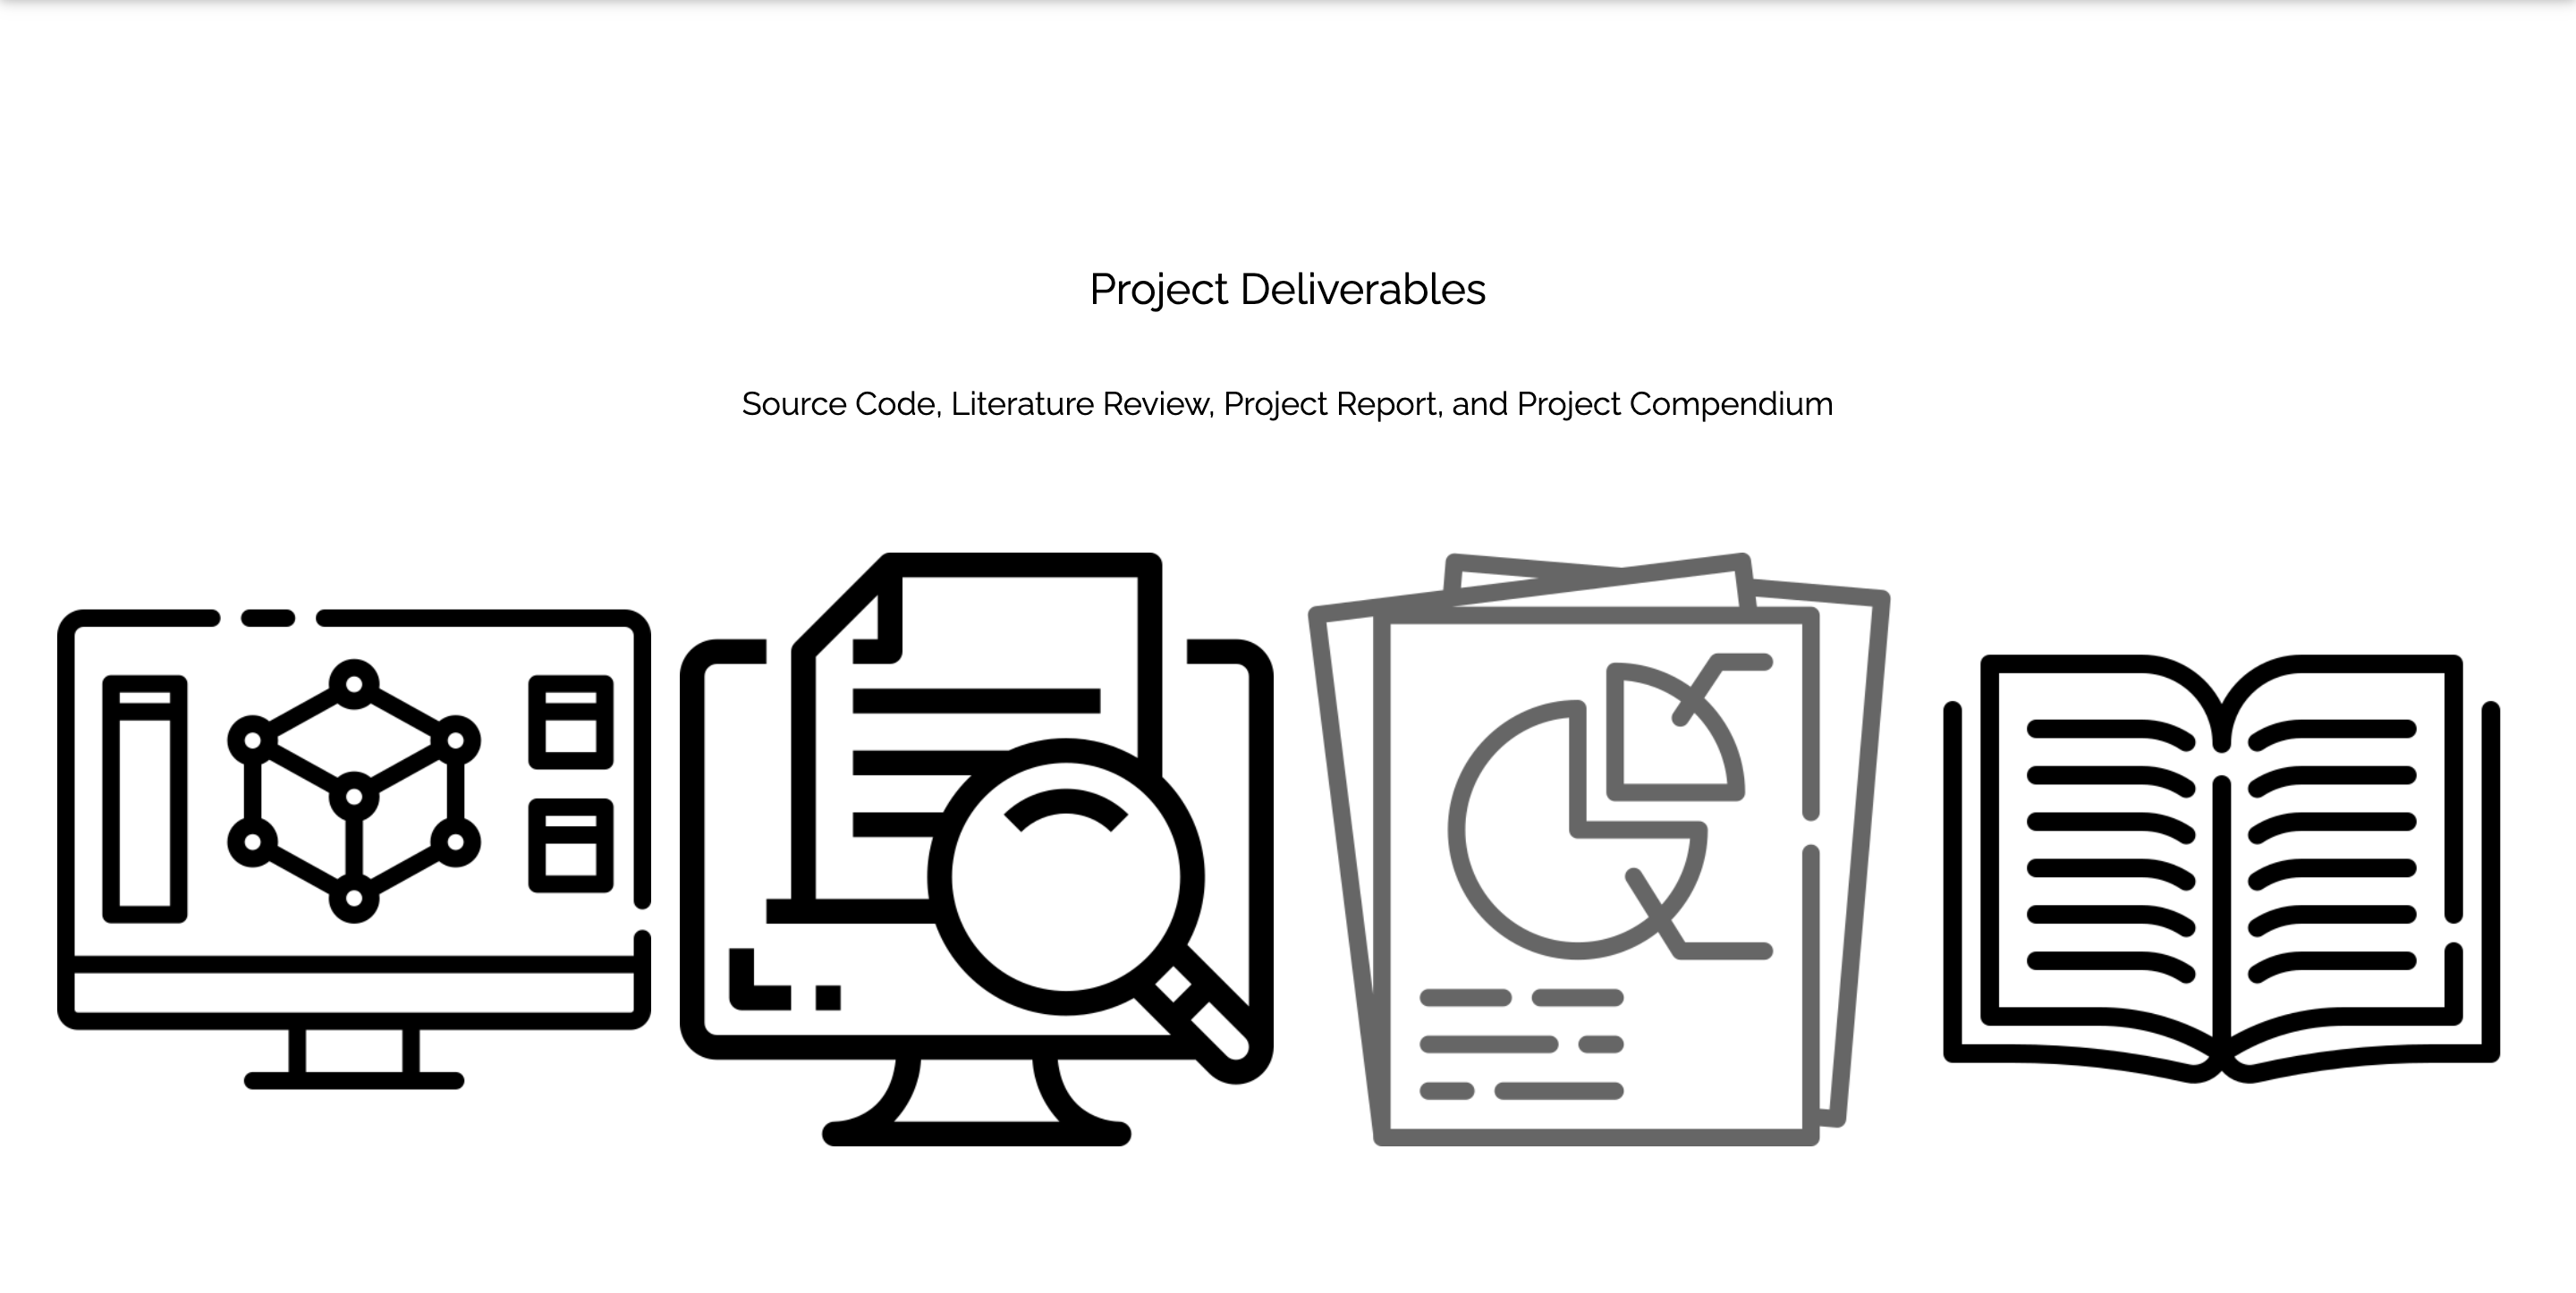
\includegraphics[width=\textwidth]{W5.png}
    \caption{GOCPI Website V1}
    \label{fig:WV1}
\end{figure}
\newpage
\section{Programming}
These section contains all programming scripts for the project.
\subsection{GOCPI NZ Energy Systems Example}
\lstinputlisting[language=Python]{"/Users/connor/Google Drive/Documents/University/Courses/2020/ENGSCI 700A&B/GOCPI/src/GOCPI_NZ_Example.gyp"}
The GOCPI NZ Energy Systems Example is the processing script for designing NZ and AUS Energy Systems
\subsection{GOCPI Module}
\subsubsection{Navigation}
The module to provide navigation functionalities to access files in directories.
\lstinputlisting[language=Python]{"/Users/connor/Google Drive/Documents/University/Courses/2020/ENGSCI 700A&B/GOCPI/src/GOCPI/GOCPI/Navigation.py"}
\subsubsection{Energysystems}
The module to load in existing energy systems to create model and data files.
\lstinputlisting[language=Python]{"/Users/connor/Google Drive/Documents/University/Courses/2020/ENGSCI 700A&B/GOCPI/src/GOCPI/GOCPI/Energysystems.py"}
\subsubsection{CreateCases}
The module to create user-defined energy systems.
\lstinputlisting[language=Python]{"/Users/connor/Google Drive/Documents/University/Courses/2020/ENGSCI 700A&B/GOCPI/src/GOCPI/GOCPI/CreateCases.py"}
\subsubsection{Forecasting}
The module to forecast energy and finance-related values.
\lstinputlisting[language=Python]{"/Users/connor/Google Drive/Documents/University/Courses/2020/ENGSCI 700A&B/GOCPI/src/GOCPI/GOCPI/Forecasting.py"}
\subsubsection{Optimisation}
The module to solve energy systems either locally or remotely using IBM technologies.
\lstinputlisting[language=Python]{"/Users/connor/Google Drive/Documents/University/Courses/2020/ENGSCI 700A&B/GOCPI/src/GOCPI/GOCPI/Optimisation.py"}

\section{Development Scripting}
The scripts within this section were used to design the GOCPI modules needed for the project.
\subsection{GOCPI Data Cases}
This script helped set the structure to build the model and data files for energy systems.
\lstinputlisting[language=Python]{"/Users/connor/Google Drive/Documents/University/Courses/2020/ENGSCI 700A&B/GOCPI/src/GOCPI_Data_Cases.gyp"}
\subsection{GOCPI Energy Balances}
This script helped extract energy balances from the International Energy Agency's World Energy Balances.
\lstinputlisting[language=Python]{"/Users/connor/Google Drive/Documents/University/Courses/2020/ENGSCI 700A&B/GOCPI/src/GOCPI_EB.gyp"}
\subsection{GOCPI Geographies}
This script helped create the geographical subsets for modelling energy regions.
\lstinputlisting[language=Python]{"/Users/connor/Google Drive/Documents/University/Courses/2020/ENGSCI 700A&B/GOCPI/src/GOCPI_Geographies.gyp"}
\subsection{GOCPI Inputs}
This script helped update values in the Excel spreadsheet when developing a standardised modelling process for the TIMES Methodology.
\lstinputlisting[language=Python]{"/Users/connor/Google Drive/Documents/University/Courses/2020/ENGSCI 700A&B/GOCPI/src/GOCPI_Inputs.gyp"}
\subsection{GOCPI Model Import}
This script helped import OseMOSYS models.
\lstinputlisting[language=Python]{"/Users/connor/Google Drive/Documents/University/Courses/2020/ENGSCI 700A&B/GOCPI/src/GOCPI_Model_Import.gyp"}
\subsection{GOCPI Optimisation}
This script helped incorporate IBM optimisation technologies into the package.
\lstinputlisting[language=Python]{"/Users/connor/Google Drive/Documents/University/Courses/2020/ENGSCI 700A&B/GOCPI/src/GOCPI_Optimisation.gyp"}

\section{OseMOSYS}
This section displays the text files formulated to create the lp file.
These are formulated using Python-based processing scripts and the GOCPI Energysystems module.
\subsection{Model File}
\lstinputlisting{"/Users/connor/Google Drive/Documents/University/Courses/2020/ENGSCI 700A&B/GOCPI/data/Inputs/GOCPI OseMOSYS/GOCPI_OseMOSYS_Model.txt"}
\subsection{Data File}
This data file is created from a partially complete NZ/AUS Energy system.
The file shows the complexity of energy modelling and creating user-defined energy systems.
The parameters to be modelled are mostly denoted by binary values.
\lstinputlisting{"/Users/connor/Google Drive/Documents/University/Courses/2020/ENGSCI 700A&B/GOCPI/data/Inputs/GOCPI OseMOSYS/GOCPI_OseMOSYS_Data.txt"}
\subsection{Linear Programme File}
This file is the lp formulation required to use CPLEX.
The file is not included in this compendium as the Utopian example is nearly 1.2 million lines of code.

\section{Project Log Book}
Disclaimer: Contributions to the Project Log Book grew inconsistent toward the later stages of the project.
\subsection*{January - February}
\begin{itemize}
	\item Began scoping energy related project during experience in the Commercial team at ExxonMobil Australia
	\item Emailed and Meet with Rosalind
	\item Decided to look at Carbon Pricing Initiatives to inform reinvestment and carbon pricing initiatives
	\item Rosalind tasked with with investigating GAMS
\end{itemize}
\subsection*{March 1st - May 30th}
\begin{itemize}
	\item Coronavirus was classified a worldwide pandemic
	\item New Zealand was sent into lockdown
	\item Researched 30+ Academic reports, articles, websites for Literature Review
	\item Wrote 10 page Literature Review
	\item Scoped the project
	\item Submitted Mid-Semester Literature Review on May 5th
	\item Installed GAMS on my local device
	\item Began researching the construction of an energy system with Excel, VEDA FE, GAMS, VEDA BE, Python
	\item Created GOCPI Geographies.gyp script to combined cities, countries and continents while providing granularity to the modelling process
	\item Created GOCPI.html as a project display for selling the project
	\item Ran into a series of installation and usage issues with VEDA and GAMS
	\item Requested VM to work from home
	\item Installed VMware and GAMS on FlexIT systems
	\item Faced GAMS Licensing issues on FlexIT
\end{itemize}
\subsection*{May 31st 2020}
\begin{enumerate}
	\item Installed Microsoft Remote Desktop and FortiClient VPN to access UoA Virtual Machine
	\item Set up Virtual Machine
\end{enumerate}
\subsection*{June 1st 2020}
\begin{enumerate}
	\item Installed VEDA FE and VEDA FE on Virtual Machine
	\item Downloaded 12 Demo Models to build my TIMES Model
\end{enumerate}
\subsection*{June 3rd}
\begin{enumerate}
	\item Begun testing the Model the Demo Models
\end{enumerate}
\subsection*{June 4th - June 10th}
\begin{enumerate}
	\item Meeting with Rosalind. Discussed set up and action points moving forward.
	\item Showed VEDA-FE. Four assessments were discussed.
	\item Continued researching how to use VEDA
\end{enumerate}
\subsection*{June 11th - Approximately 4 hours}
\begin{enumerate}
	\item Meeting with Rosalind at 10:30am via Zoom
	\item Discussed action points moving forward.
	\item Continued to adapt excel spreadsheets for Excel Data.
	\item There is still an issue with GAMS Installation (Check with Tony. He knows a guy)
	\item VEDA FE creates the necessary DD files. Continue to work through the DEMO Models to understand GAMS.
\end{enumerate}
\subsection*{June 16th - July 1st}
\begin{itemize}
	\item No Progress - Study Break and Exams for ACCTG 371, FINANCE 362 and ENGSCI 711
\end{itemize}
\subsection*{July 2nd}
\begin{itemize}
	\item Last meeting in Rosalind's corner office. Discussed online exams, Chegg, cheating and project next steps.
	\item Agreed to adapt spreadsheets for user input and use BP's World Energy Outlook Statistics to determine production, conversion and consumption rates.
\end{itemize}
\subsection*{July 3rd}
\begin{itemize}
	\item Began adapting Demo 12 model for custom inputs
	\item Began using the openpyxl python library to manipulate excel (GOCPI Input.gyp)
\end{itemize}
\subsection*{July 4rd}
\begin{itemize}
	\item Continue to work on openpyxl adaptation with xls and xlsx excel sheets
\end{itemize}
\subsection*{July 6th}
\begin{itemize}
	\item Created a proper file directory for managing the project
	\item Continued to adapt GOCPI Inputs.gyp to scale across multiple sheets
	\item Adapted GOCPI.html, GOCPI Inputs.gyp and GOCPI Geographies to work after rearranging the geographies
	\item Nearly had a heart attacked as I was led to believe issues with Github and Git meant I deleted my entire project
	\item Recovered entire project and reports
\end{itemize}
\subsection*{July 7th}
\begin{itemize}
	\item Worked on file manipulation in Google Drive via Google Cloud APIs
	\item Discovered IEA Energy Balances on stats.OECD.org via Uni library databases
	\item Found 20GB csv on Energy Balances data
	\item Processed 20GB csv to create two ~80MB csv for 2017 energy balance data using Microsoft Access
\end{itemize}
\subsection*{July 7th}
\begin{itemize}
	\item Developed and resolved issues relating to git and Github
	\item Developed processing methods for Energy Balance statistics using pandas pivot table function
\end{itemize}
\subsection*{July 17th}
\begin{itemize}
	\item Meeting with Kiti (NZ TIMES Energy Modeler)
	\item Discuss constraints associated TIMES and GAMS modelling
	\item Introduced to OseMOSYS (Open Source, Energy Modelling Tool)
	\item Introduced to MBIE,EECA (https://www.eeca.govt.nz/)
	\item Agreed to explore OseMOSYS and alternative datasources to build an alternative product.
	\item Agreed to keep Kiti updated on projec process moving forward.
\end{itemize}
\subsection*{July 18th}
\begin{itemize}
	\item Downloaded MBIE Energy 
	\item Research OseMOSYS energy modelling Approach
	\item Downloaded OseMOSYS energy modelling tools
	\item Tested Pyomo, GNU and GAMS approaches. GNU optimised using glpsol in conda environment. Progress works well.
	\item Decision: Move away from TIMES/GAMS modelling to using Osemosys.
	\item Began Scripting Sheet to generate model input text file
\end{itemize}
\subsection*{July 19th}
\begin{itemize}
	\item Created excel spreadsheet to store OseMOSYS energy model inputs
	\item Began adapting sets, parameters, variables, equations and constraints to excel template.
	\item Researched more about OseMOSYS
\end{itemize}
\subsection*{July 20th}
\begin{itemize}
	\item Continued to adapt 200+ lines of model code in the excel templates
\end{itemize}
\subsection*{July 21st}
\begin{itemize}
	\item Learned to create custom python packages.
	\item Began working on adjustable sets
\end{itemize}
\subsection*{July 22nd}
\begin{itemize}
	\item 
\end{itemize}
\subsection*{July 23rd}
\begin{itemize}
	\item Productive meeting with Rosalind, showed model output. (Rosalind said progress was really exciting)
\end{itemize}
\subsection*{July 24th}
\begin{itemize}
	\item Continued creating a custom package for the GCOPI module.
\end{itemize}
\subsection*{July 25th}
\begin{itemize}
	\item Started GOCPI module to create scalable data files
\end{itemize}
\subsection*{July 26th}
\begin{itemize}
	\item Continued to adapt GOCPI custom package to create scalable data files (Completed)
\end{itemize}
\subsection*{July 27th}
\begin{itemize}
	\item Edited report headings and created a structure for the Research Report.
\end{itemize}
\subsection*{July 28th}
\begin{itemize}
	\item Investigated CPLEX Solvers
	\item Registered for the IBM Academic Initiative
	\item Downloaded and Installed IBM ILOG CPLEX Optimizer Studio
	\item Installed cplex and docplex Python APIs from the IBM ILOG CPLEX Optimizer Studio
	\item Added create model file model to GOCPI
\end{itemize}
\subsection*{July 30th - August 9th}
\begin{itemize}
	\item Spent a day fixing git commit and push issues
	\item Installed GIT LFS and the functionality of .gitignore to prevent the committing .mp4 and .lp files
	\item Installed yapf in Microsoft Visual Studio Code to enable PEP-8 Autoformatting
	\item Wrote 4.5 pages for the technical, mainly focusing on the setup of Python, Anaconda, CPLEX, Git, GitHub, folder structure suggested by Wilson et al and the OseMOSYS methodology.
	\item Submitted the 4-6 page technical report.
	\item Created presentation structure 
\end{itemize}
\subsection*{August 10th}
\begin{itemize}
	\item Drafted and submitted four slide summary for presentation.
	\item Recorded and submitted 5 minute presentation
\end{itemize}
\subsection*{August 12th}
\begin{itemize}
	\item Lockdown and Became Ill
	\item Went and got COVID-19 Testing (Stood in Queue for 4.5 hours)
\end{itemize}
\subsection*{August 13th}
\begin{itemize}
	\item Very productive meeting with Rosalind
	\item Discussed project process, presentation and mid-year technical report
	\item Continuing doing what I am doing.
	\item Continued developing NZ Example
	\item Abandoned developing the NZ Example as faced severe limitations
	\item Continued developing the Navigation, Forecasting, Energysystems and CreateCases modules.
\end{itemize}
\subsection*{September 2nd - September 30th}
\begin{itemize}
	\item IBM Cloud Installation and Application.
	\item Discussed project process, presentation and mid-year technical report
	\item Investigated adopting DOCPLEX optimisation technologies.
	\item Discovered limitations in the IBM Decision Optimisation service. This was no longer viable as imported to IBM Watson Machine Learning service.
	\item Began exploring the implementation of the IBM Watson Machine Learning service to engage with this pipeline.
	\item Developed the optimisation module to use
\end{itemize}
\subsection*{October 1st - October 29th}
\begin{itemize}
	\item Systems week interfered with the construction of the report.
	\item Wrote the report
	\item Edited the report
	\item Reviewed the report
	\item Had three productive meetings with my supervisor about the report.
\end{itemize}
\subsection*{October 30th}
\begin{itemize}
	\item Submitted the final report
\end{itemize}
\section{Bibliography}
\printbibliography
\end{document}